\documentclass{article}
\usepackage[utf8]{inputenc}
\usepackage{graphics}
\usepackage{amsmath}
\usepackage{amssymb}
\usepackage{cases}
\usepackage{graphicx}
\title{5V Charger Lab Report}
\author{Aditya Gangula EP20BTECH11001}

\begin{document}

\maketitle

\section*{Circuit and Component description}
The circuit includes
\begin{itemize}
    \item 12-0-12 step down transformer
    \item 4 Si diodes connected to form a full bridge rectifier
    \item Capacitor for smoothing
    \item 7805 regulator
\end{itemize}
\begin{figure}
    \centering
    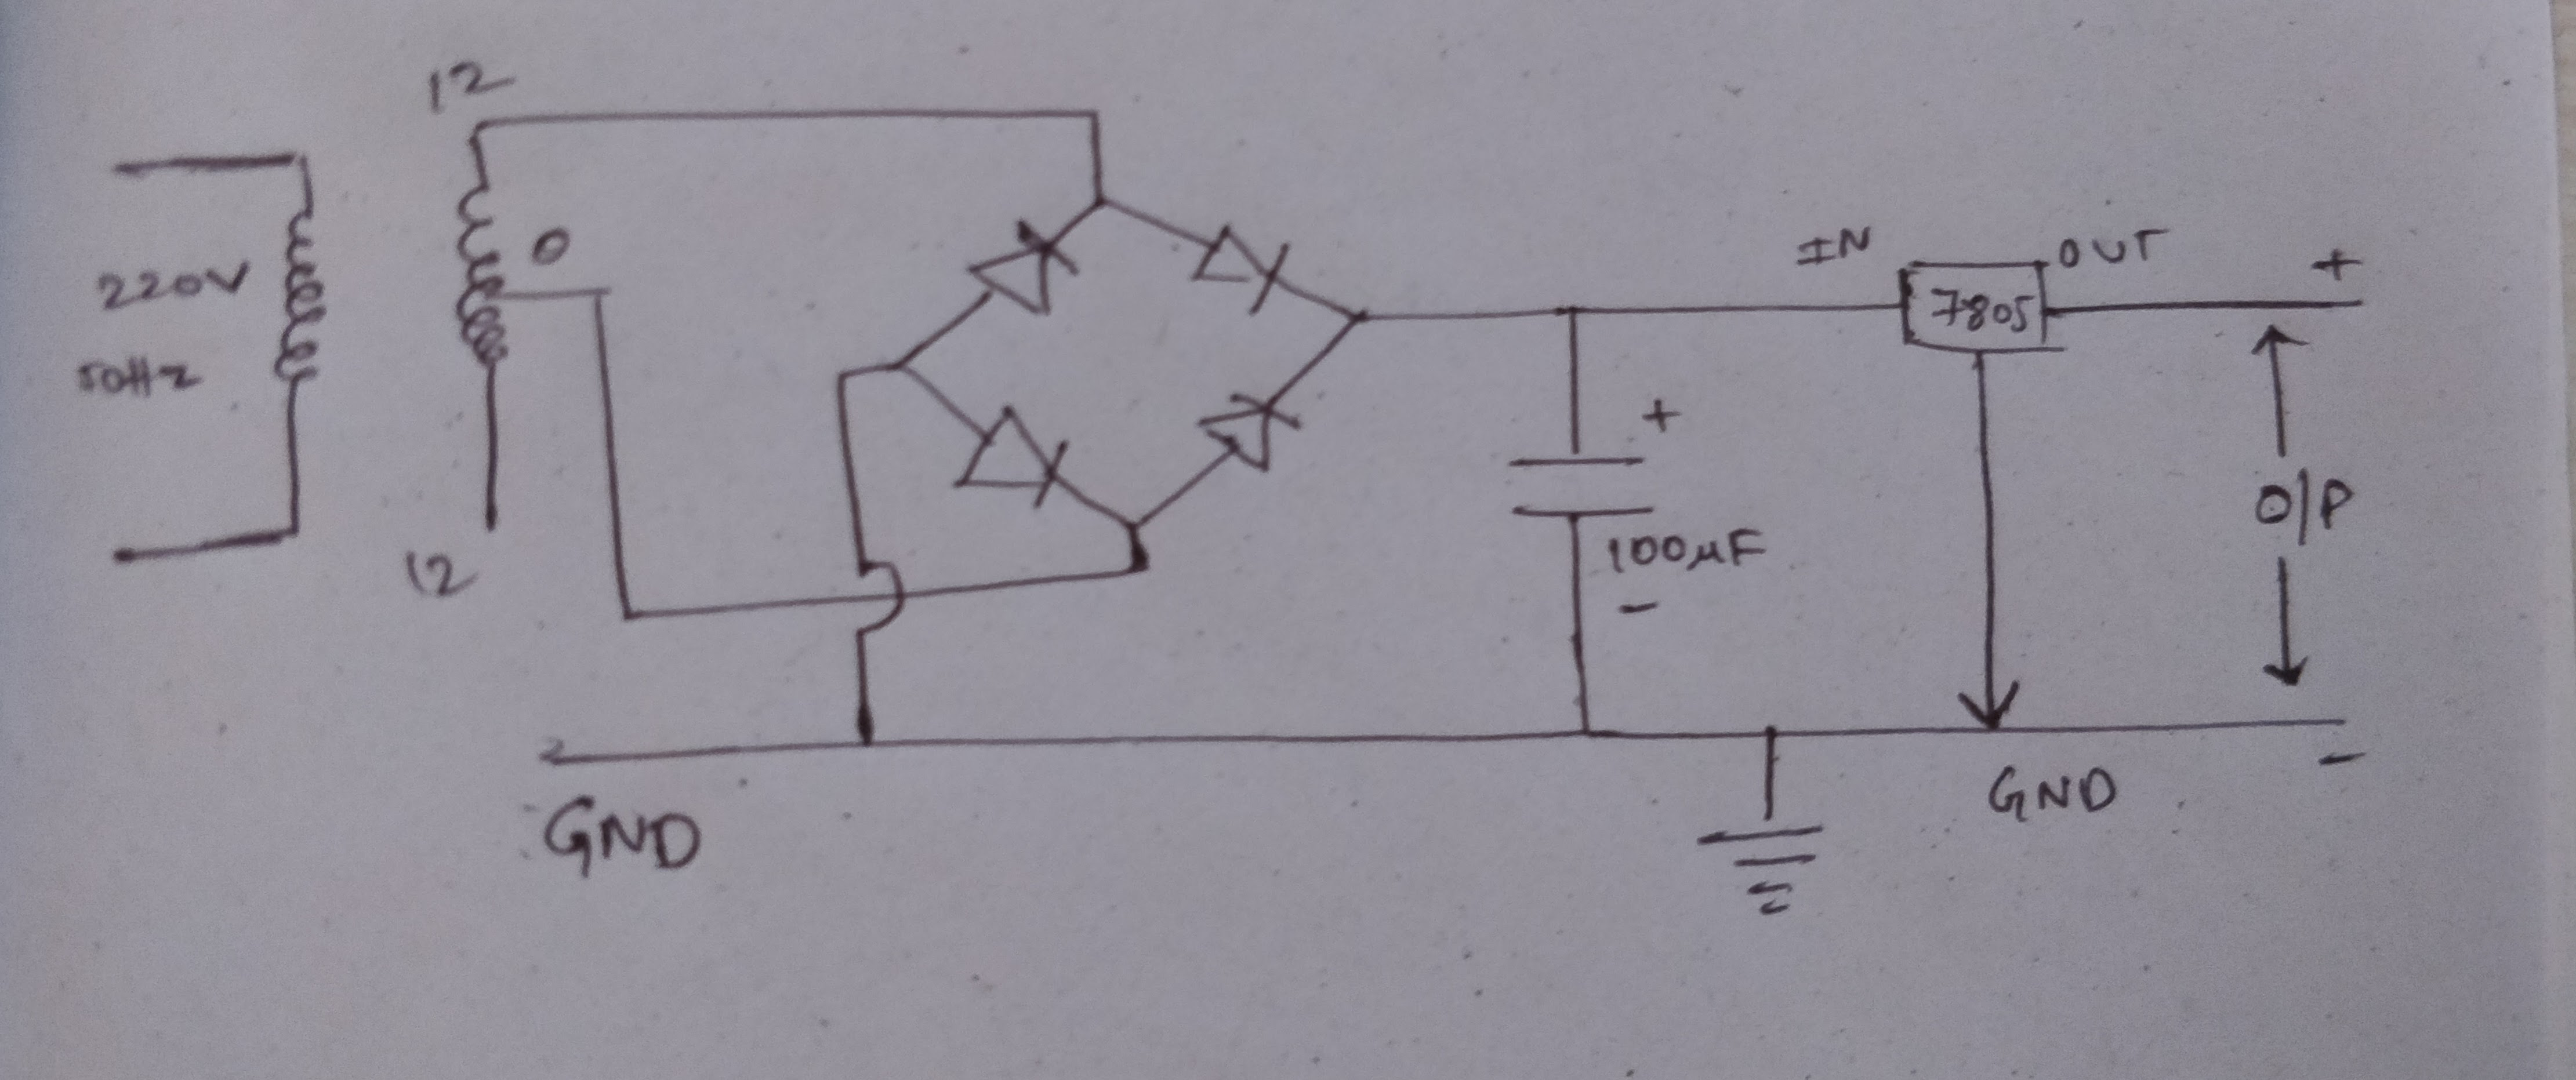
\includegraphics[width=\columnwidth]{figs/circuit.png}
    \caption{Circuit}
    \label{fig:circ}
\end{figure}
The step-down transformer converts the the input 220V 50Hz AC signal into a 12V 50Hz AC signal which looks like as shown in fig 2.\\
\begin{figure}[!h]
    \centering
    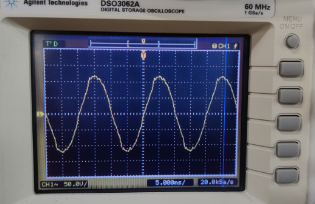
\includegraphics[width=\columnwidth]{figs/trans.png}
    \caption{Transformer output}
    \label{fig:my_label}
\end{figure}
The full bridge rectifier, which is made by arranging the diodes as shown in the circuit figure, converts the signal into a rectified 12V 100Hz signal. The 100$\mu$F capacitor charges due to the rectified signal and as the signal drops it discharges slow enough to maintain nearly the same voltage output until the peak of the rectified signal is attained again.\\
\begin{figure}
    \centering
    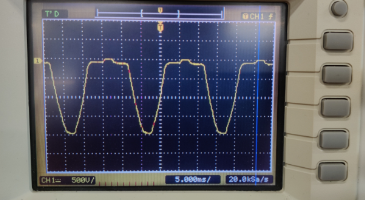
\includegraphics[width=\columnwidth]{figs/rect.png}
    \caption{Rectified signal}
    \label{fig:my_label}
\end{figure}
\begin{figure}
    \centering
    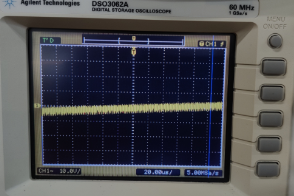
\includegraphics[width=\columnwidth]{figs/cap.png}
    \caption{Across capacitor 18V output}
    \label{fig:my_label}
\end{figure}
The 7805 regulator produces an output of constant 5V DC from an input of 12V DC.\\
\begin{figure}
    \centering
    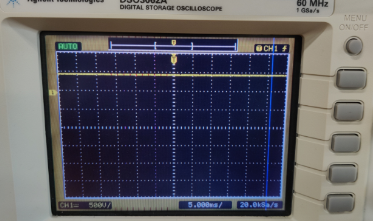
\includegraphics[width=\columnwidth]{figs/dc.png}
    \caption{DC output}
    \label{fig:my_label}
\end{figure}
\begin{figure}
    \centering
    \includegraphics[width=\columnwidth]{figs/output.png}
    \caption{Final output}
    \label{fig:my_label}
\end{figure}
\end{document}
